\documentclass[tikz,convert={outfile=\jobname.svg}]{standalone}
\usepackage{tikz}
\usepackage{pagecolor}
\usetikzlibrary{arrows,shapes.geometric,arrows.meta,calc,chains,scopes,shapes.misc,backgrounds}
\pgfdeclarelayer{background}
\pgfdeclarelayer{foreground}
\pgfsetlayers{background,main,foreground}
\pagecolor{white}

\tikzset{ 
   line/.style  = {-, line width=0.5mm, },
   arrow/.style = {-latex,line width=0.5mm, }, 
   doublearrow/.style = {latex-latex,line width=0.5mm, },  
}

\begin{document}
   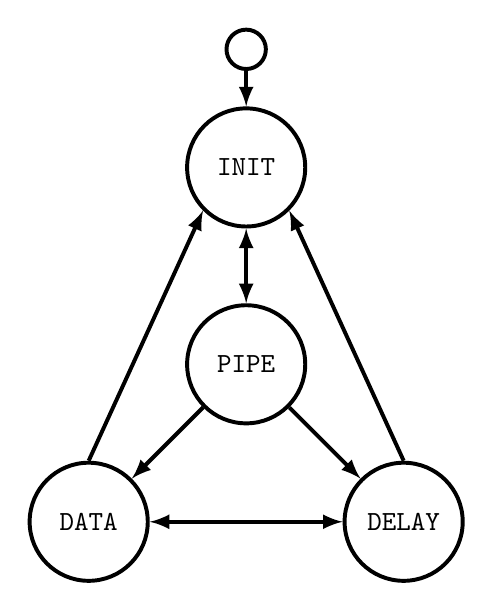
\begin{tikzpicture} 
     
      \node[
         circle,
         draw,
         font=\ttfamily,
         line width = 0.5mm,
         minimum height=5mm,
         minimum width=5mm,
      ] (reset) at (0mm,15mm){};
      
      \node[
         circle,
         draw,
         font=\ttfamily,
         line width = 0.5mm,
         minimum height=15mm,
         minimum width=15mm,
      ] (init) at (0mm,0mm){INIT};

      \node[
         circle,
         draw,
         font=\ttfamily,
         line width = 0.5mm,
         minimum height=15mm,
         minimum width=15mm,
      ] (pipe) at (0mm,-25mm){PIPE};
       
      \node[
         circle,
         draw,
         font=\ttfamily,
         line width = 0.5mm,
         minimum height=15mm,
         minimum width=15mm,
      ] (data) at (-20mm,-45mm){DATA};
      
      \node[
         circle,
         draw,
         font=\ttfamily,
         line width = 0.5mm,
         minimum height=15mm,
         minimum width=15mm,
      ] (delay) at (20mm,-45mm){DELAY};
      
      \draw[arrow]       (reset.south)      -- (init.north);
      \draw[doublearrow] (init.south)       -- (pipe.north);
      \draw[arrow]       (pipe.south west)  -- (data.north east);
      \draw[arrow]       (pipe.south east)  -- (delay.north west);
      \draw[doublearrow] (data.east)        -- (delay.west);
      \draw[arrow]       (data.north)       -- (init.south west);
      \draw[arrow]       (delay.north)      -- (init.south east);
   \end{tikzpicture}
\end{document}
